\documentclass[10pt,a4paper]{article}
\usepackage[latin1]{inputenc}
\usepackage{amsmath}
\usepackage{amsfonts}
\usepackage{amssymb}
\usepackage{graphicx}
\usepackage{geometry}
\usepackage{tikz}
\usepackage{amsthm}

\geometry{a4paper, top=25mm, left=40mm, right=25mm, bottom=30mm,
	headsep=10mm, footskip=12mm}
\title{statistisches Lernen\\ \large{Vorlesung Wintersemester 17/18}}

\def\firstcircle{(0,0) circle (1.5cm)}
\def\secondcircle{(45:2cm) circle (1.5cm)}
\def\thirdcircle{(0:2cm) circle (1.5cm)}
\date{}

\theoremstyle{definition}
\newtheorem{exmp}{Beispiel}[section]
\begin{document}
	\maketitle
	\section{Einf�hrung}
	\subsection{Vorbemerkungen}
	\begin{itemize}
		\item Bei statistischem Lernen geht es darum intelligente Schl�sse aus Daten zu ziehen
		\begin{itemize}
			\item Fokus auf Methoden zu Analysen
			\item wenig/nicht �ber Design
			\item viele Bsp. aus dem Bereich der klinischen Studien
			\item Anwendungen auf ganz anderen Gebieten
		\end{itemize}
	\item Beispielhafte Anwendungen
	\begin{itemize}
		\item Unterscheiden sich Behandlungen A und B
		\item Was sind die Eigenschaften eines diagnostischen Test
		\item Gibt es einen Zusammenhang zwischen Krankheiten A und B
	\end{itemize}
	\end{itemize}
\subsection{Wahrscheinlichkeit}
\subsubsection{Zug�nge}
\begin{itemize}
	\item relative H�ufigkeit (frequentistisch)
	\item Ma� f�r eine �berzeugung (Bayes'sche Statistik)
\end{itemize}
\textbf{frequentistisch:} intuitiv, basiert auf wiederholbaren ''Experimenten'' (z.B. M�nzwurf, radioaktiver Zerfall, Schwangerschaft bei Kontrazeptionsmethode(Verh�tungsmethode) A, 5-Jahre �berleben nach Chemotherapie, Regen am n�chsten Tag in Leipzig)

\begin{itemize}
	\item in den ersten Vorlesungen folgen wir einem theoretischen Zugang
	\begin{itemize}
		\item dadurch bekommt man ein solides Fundament
		\item wir werden nicht mathematisch streng sein k�nnen, (Stichwort Kolmogorow Axiomatik)
	\end{itemize}
\end{itemize}
\subsubsection{Das Ereignisfeld}
\begin{itemize}
	\item als \textit{Ereignis} bezeichnet man einen m�glichen Ausgang eines ''Zufallsexperimentes'', z.B. ''Zahl liegt oben''
	\item Ein System hei�t \textit{Ereignisfeld}, wenn:
	\begin{itemize}
		\item es das sichere und das unm�gliche Ereignis enth�lt

				\item A und B teil eines Systems sind, dann auch $AB$ ($A\cap B$) ''Produkt'' von A und B, bedeutet $x \in A \text{ und } B$
			\item $A+B$ ($A \cup B$) ''Summe'', mindestens eines der Ereignisse A und B tritt ein
			\item $A-B$ ($A\backslash B$) "Differenz'' A tritt ein, w�hrend B nicht eintritt

	
	\end{itemize}
\end{itemize}
\begin{exmp}
	M�nzwurf Ereignisfeld \{A,B,$\Omega$, $\emptyset$\}\\
	A - Zahl oben\\B - Wappen oben \\ $\Omega$ - Zahl oder Wappen oben \\ $\emptyset$ - weder Zahl noch Wappen oben
\end{exmp}

\subsubsection{Gesetze der Ereignisse}
\begin{itemize}
	\item Kommutativ: $A+B = B+A$, $AB = BA$
	\item Assoziativ: $A+(B+C)$ = $(A+B)+C$; $A(BC) = (AB)C$
	\item Distributiv: $A(B+C)$ = $(AB)+(AC)$; $A+(BC) = (A+B)(A+C)$ *
	\item Identit�ten: $A+A = A$; $AA = A$
\end{itemize}
*(A+B)(A+C) = AA+AC+BA+BC = A+(BC)

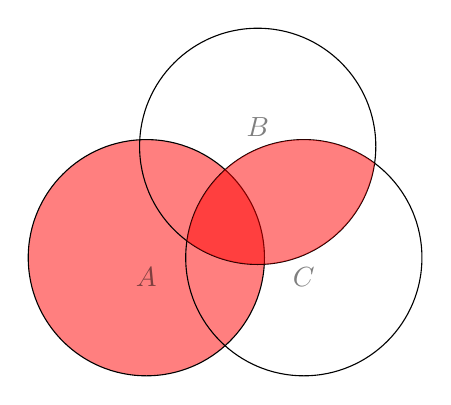
\begin{tikzpicture}
\begin{scope}[shift={(3cm,-5cm)}, fill opacity=0.5]
\fill[red] \firstcircle;

\draw \firstcircle node[below] {$A$};
\draw \secondcircle node [above] {$B$};
\draw \thirdcircle node [below] {$C$};

\clip \secondcircle;
\clip \thirdcircle;
\fill[red]\thirdcircle;
\end{scope}
\end{tikzpicture}

\subsubsection{Wahrscheinlichkeitsbegriff}
Axiom 1: Jedem Ereignis $A$ aus dem Ereignisfeld $F$ ordnet maneine nichtnegative Zahl $P(A)$ zu. Das ist die \textit{Wahrscheinlichkeit}.
Axiom 2: $P(\Omega)=1$
Axiom 3: Sind Ereignisse $A_i$ $i\in {1,..,n}$ paarweise unvereinbar, d.h: $A_I A_J = \emptyset$ mit $i != j $ so gilt $P(A_1+A_2+ \ldots A_n) = P(A_1+P(A_2)+\ldots+P(A_n) ) $ So folgen folgende Eigenschaften f�r Wahrscheinlichkeiten
\begin{itemize}
	\item $P(\emptyset)= 0$
	\item $P(\neg A) = 1 - P(A)$, $\neg A = \Omega -A$
	\item $ 0 \leq P(A) \leq 1$
	\item F�r $A \subset B$ (A ist Teilereignis von B) folgt $P(A) \leq P(B)$
	\item $P(A+B) = P(A)+P(B)-P(AB)$
	\item  $P(A_1 + A_2+ \ldots +A_n) \leq P(A_1) + P(A_2)+ \ldots+P(A_n)$
\end{itemize} 
\subsubsection{Bedingte Wahrscheinlichkeit}
Eine Wahrscheinlichkeit von A unter der BEdingung dass B eingetrteten ist schreibt man als $PA|B)$
\[P(A|B) = \frac{P(AB)}{P(B)}\]
\end{document}